% =============================================================================
% V. Experimental Setup and Results — AC-DSGF
% Soft Comm. Mass naming; scalability/deployment = theory validation (not extras)
% =============================================================================

\section{Evaluation under Communication-Constrained Swarm Coordination}
\label{sec:setup}

We evaluate whether AC-DSGF can \textbf{maintain comparable task performance}
while \textbf{learning a scalable sparse communication topology}.
Success alone is not the primary score; we jointly report Success, Soft
Comm.\ Mass, CEI, and density scaling $\eta_N$.

\subsection{Environment and Protocol}
All formal results use the VMAS continuous multi-agent \texttt{navigation}
scenario.
Unless stated otherwise:
\begin{itemize}
  \item Training: $102{,}400$ frames; evaluation uses TorchRL rollouts with
        \texttt{step\_mdp} after \texttt{env.step}.
  \item Main comparison: $N{=}16$; $R_c{=}0.5$; horizon $H{=}128$;
        success threshold $0.3$.
  \item DSGF~v2 backbone and AC hyperparameters are frozen
        (\texttt{dsgf\_v2\_frozen.yaml}, \texttt{ac\_dsgf\_16uav.yaml}).
\end{itemize}

\subsection{Baselines}
MAPPO (no graph messaging);
GAT-MAPPO (binary radius graph + alignment reward);
Transformer / full attention;
DSGF~v2 (quality-weighted sparse graph + residual);
\textbf{AC-DSGF} (learned gate + budget + residual).

\subsection{Metrics}
Success $S$, Soft Communication Activation Mass $C$
(Eq.~\eqref{eq:comm-cost}),
$\mathrm{CEI}=S/(C+\varepsilon)$ (Eq.~\eqref{eq:cei}),
and normalized density $\eta_N=C/(N(N-1))$.

\subsection{Experiment Map}
\begin{enumerate}
  \item \textbf{Overall performance} (Table~\ref{tab:main}): Success / Soft Mass / CEI.
  \item \textbf{Budget \& dense saturation} (Table~\ref{tab:budget}, Fig.~\ref{fig:pareto}).
  \item \textbf{Ablation} (Table~\ref{tab:ablation}, Table~\ref{tab:silence}).
  \item \textbf{Communication behavior} (Fig.~\ref{fig:trigger}, Fig.~\ref{fig:gate-stable}).
  \item \textbf{Scalability \& deployment} (Sec.~\ref{sec:scale-deploy}, Fig.~\ref{fig:density-scale}--\ref{fig:topk}):
        theory-aligned density scaling, selectivity, Top-$K$ deployability.
  \item \textbf{Robustness} (Fig.~\ref{fig:packet-loss}): packet loss.
\end{enumerate}


\section{Results}
\label{sec:results}

\subsection{Overall Performance}
\label{sec:main}

\begin{table}[t]
\centering
\caption{Task performance under communication constraints ($N{=}16$,
unified \texttt{step\_mdp} protocol, budget ratio $\rho{=}1$).
AC-DSGF maintains task effectiveness with substantially lower Soft
Communication Activation Mass (higher CEI).
We do \emph{not} claim Success leadership.}
\label{tab:main}
\begin{tabular}{lccc}
\toprule
Method & Success (\%) & Soft Comm.\ Mass & CEI \\
\midrule
GAT          & $21.3$ & $44.14$ & $0.0048$ \\
DSGF         & $21.7$ & $40.29$ & $0.0054$ \\
\textbf{AC-DSGF} & $27.1$ & $\mathbf{0.0081}$ & $\mathbf{33.5}$ \\
\bottomrule
\end{tabular}
\end{table}

\noindent
\textbf{Reading Table~\ref{tab:main}.}
We do \emph{not} claim that AC-DSGF ``outperforms'' DSGF on Success.
The primary axes are Soft Comm.\ Mass and CEI under a task-effectiveness
constraint: Soft Mass drops from ${\sim}40$ to ${\sim}8\times10^{-3}$
(about \textbf{three orders of magnitude} in soft activation intensity),
while Success remains in a comparable operating regime
(Fig.~\ref{fig:pareto}).
Soft Mass is not a physical packet count.

\subsection{Ablation Study}
\label{sec:ablation}

\begin{table}[t]
\centering
\caption{DSGF residual ablation at $N{=}4$ (mechanism test; \emph{not} Table~I scale).}
\label{tab:ablation}
\begin{tabular}{lc}
\toprule
Variant & Success (\%) \\
\midrule
w/o Dynamic Graph & $0.28$ \\
w/o Temporal      & $0.86$ \\
w/o Residual      & $0.22$ \\
Full DSGF         & $\mathbf{9.27}$ \\
\bottomrule
\end{tabular}
\end{table}

Residual decoupling keeps guidance \emph{assistive}
($\sim$42$\times$ Success collapse without it).
AC gate ablations appear in Sec.~\ref{sec:silence}.

\subsection{Communication Budget Analysis}
\label{sec:budget-res}

\begin{table}[t]
\centering
\caption{Success (\%) under communication budget ratio $\rho$ ($N{=}16$).
Trends indicate graceful degradation under tighter budgets.}
\label{tab:budget}
\begin{tabular}{lccc}
\toprule
Budget $\rho$ & GAT & DSGF & AC-DSGF \\
\midrule
$100\%$ & $21.3$ & $21.7$ & $27.1$ \\
$50\%$  & $18.2$ & $21.6$ & $25.2$ \\
$10\%$  & $16.9$ & $21.7$ & $24.2$ \\
\bottomrule
\end{tabular}
\end{table}

Under a $90\%$ budget cut ($100\%\!\rightarrow\!10\%$), AC-DSGF success drops only
$\sim$11\% relatively ($27.1\!\rightarrow\!24.2$), consistent with Lemma~2.

\begin{figure}[t]
  \centering
  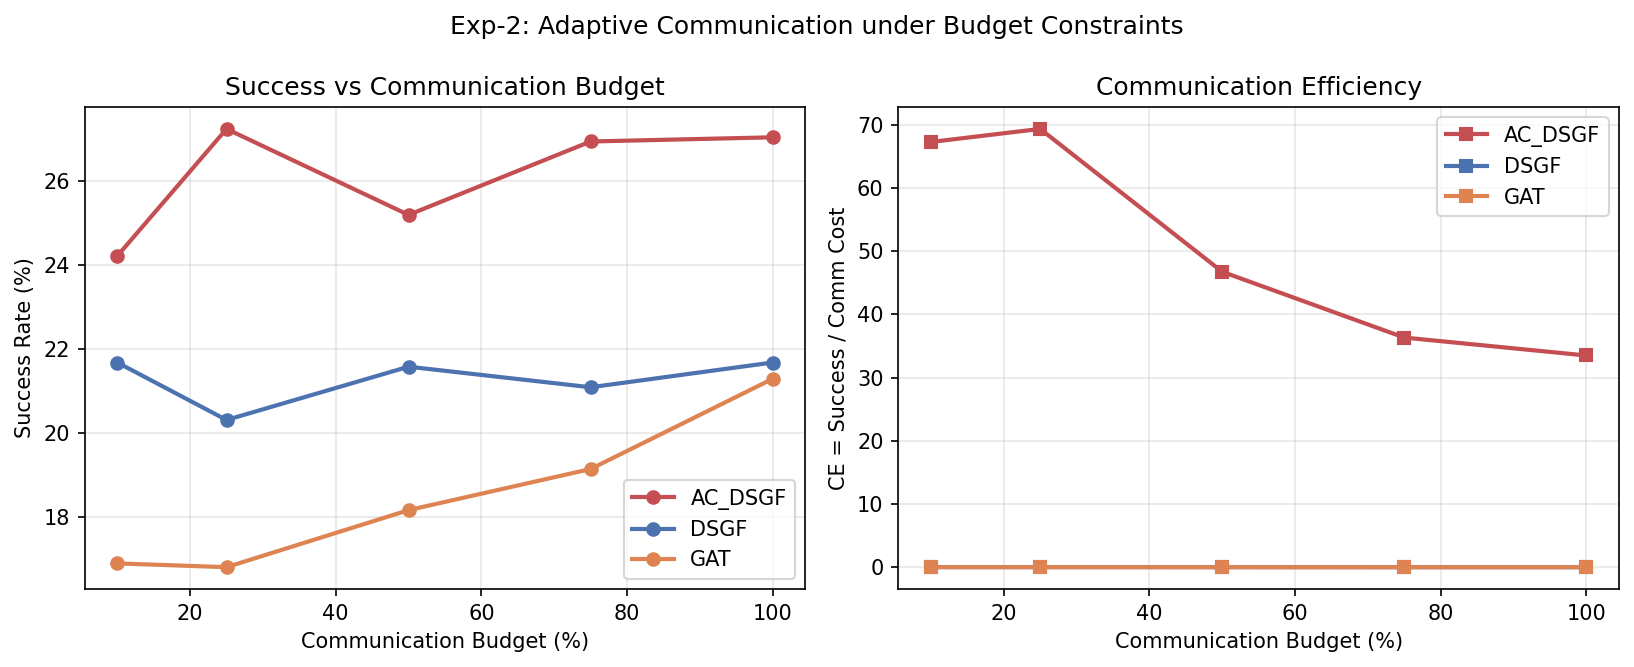
\includegraphics[width=0.92\linewidth]{figures/fig_comm_budget16.png}
  \caption{Success vs.\ communication budget ($N{=}16$).
  AC-DSGF maintains task effectiveness under severe budget cuts
  (graceful degradation).}
  \label{fig:budget}
\end{figure}

\subsection{Silence Collapse Ablation}
\label{sec:silence}

\begin{table}[t]
\centering
\caption{Communication mechanism validation ($N{=}16$, AC checkpoint).
AC-full is \emph{not} silence collapse: opening all radius edges ($g{=}A$)
inflates Soft Mass by over three orders of magnitude with only a small Success change.}
\label{tab:silence}
\begin{tabular}{lccc}
\toprule
Variant & Success (\%) & Soft Comm.\ Mass & CEI \\
\midrule
AC-full (learned) & $24.6$ & $0.008$ & $32.0$ \\
AC-no budget ($g{=}A$) & $28.9$ & $40.6$ & $0.007$ \\
AC-random gates & $28.5$ & $20.3$ & $0.014$ \\
\bottomrule
\end{tabular}
\end{table}

\noindent
Sparsity is \emph{not} silence collapse: AC-full trades a few percentage points
of Success for over-three-orders Soft Mass reduction versus full local
broadcast---selective interaction, not ``turning off communication.''

\subsection{Communication Behavior Analysis}
\label{sec:trigger}

\begin{figure}[t]
  \centering
  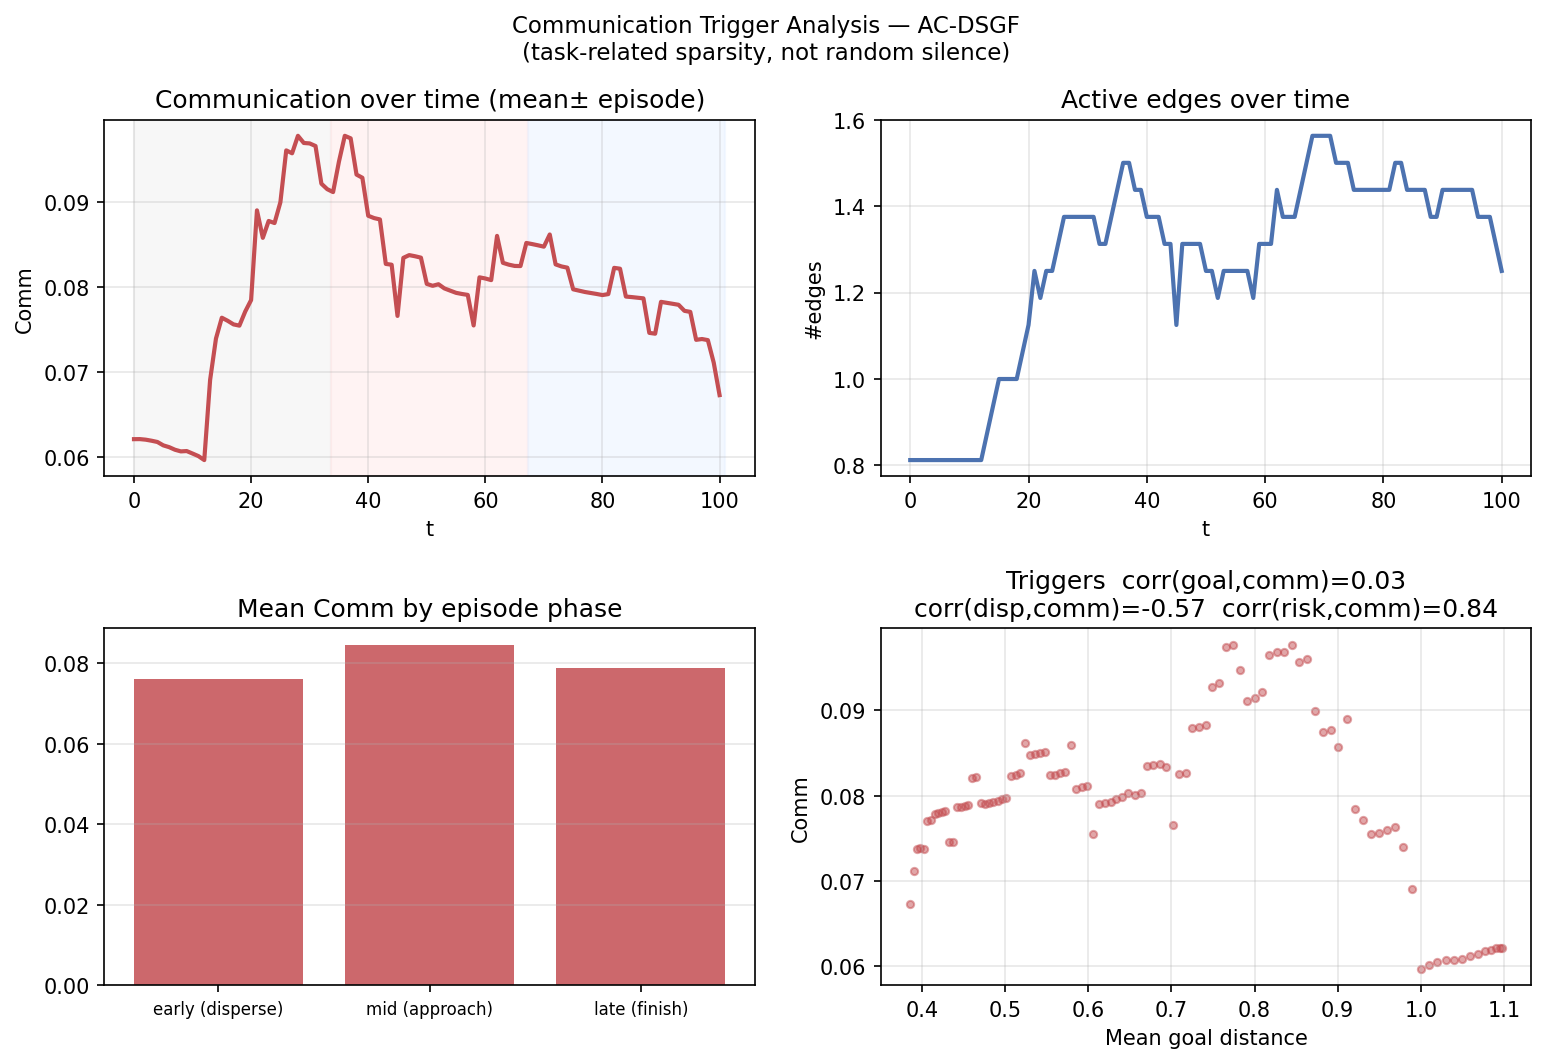
\includegraphics[width=0.95\linewidth]{figures/fig_comm_trigger.png}
  \caption{Communication behavior: Soft Mass rises with proximity risk
  ($\mathrm{corr}{=}0.84$) and falls with spatial dispersion
  ($\mathrm{corr}{=}{-}0.57$)---sparse topology is task-driven, not random.}
  \label{fig:trigger}
\end{figure}

\subsection{Scalability and Deployment Analysis}
\label{sec:scale-deploy}

This section validates Prop.~2 and deployment approximation
(Sec.~\ref{sec:theory}); it is \textbf{not} an ``additional experiment''
appendix.
Protocol: freeze an $N{=}16$ policy and zero-shot transfer to
$N\in\{8,16,32\}$ (no retraining).

\subsubsection{Communication Density Scaling}
\label{sec:density-scale}

\begin{table}[t]
\centering
\caption{Soft Comm.\ Mass $C$ and density $\eta_N=C/(N(N-1))$
(zero-shot from $N{=}16$ checkpoint).}
\label{tab:eta}
\begin{tabular}{rcccc}
\toprule
$N$ & DSGF $C$ & DSGF $\eta_N$ & AC $C$ & AC $\eta_N$ \\
\midrule
8  & $11.01$ & $0.197$ & $\mathbf{0.002}$ & $\mathbf{3.6\times10^{-5}}$ \\
16 & $22.62$ & $0.094$ & $\mathbf{0.006}$ & $\mathbf{2.5\times10^{-5}}$ \\
32 & $56.06$ & $0.057$ & $\mathbf{0.019}$ & $\mathbf{1.9\times10^{-5}}$ \\
\bottomrule
\end{tabular}
\end{table}

\begin{figure}[t]
  \centering
  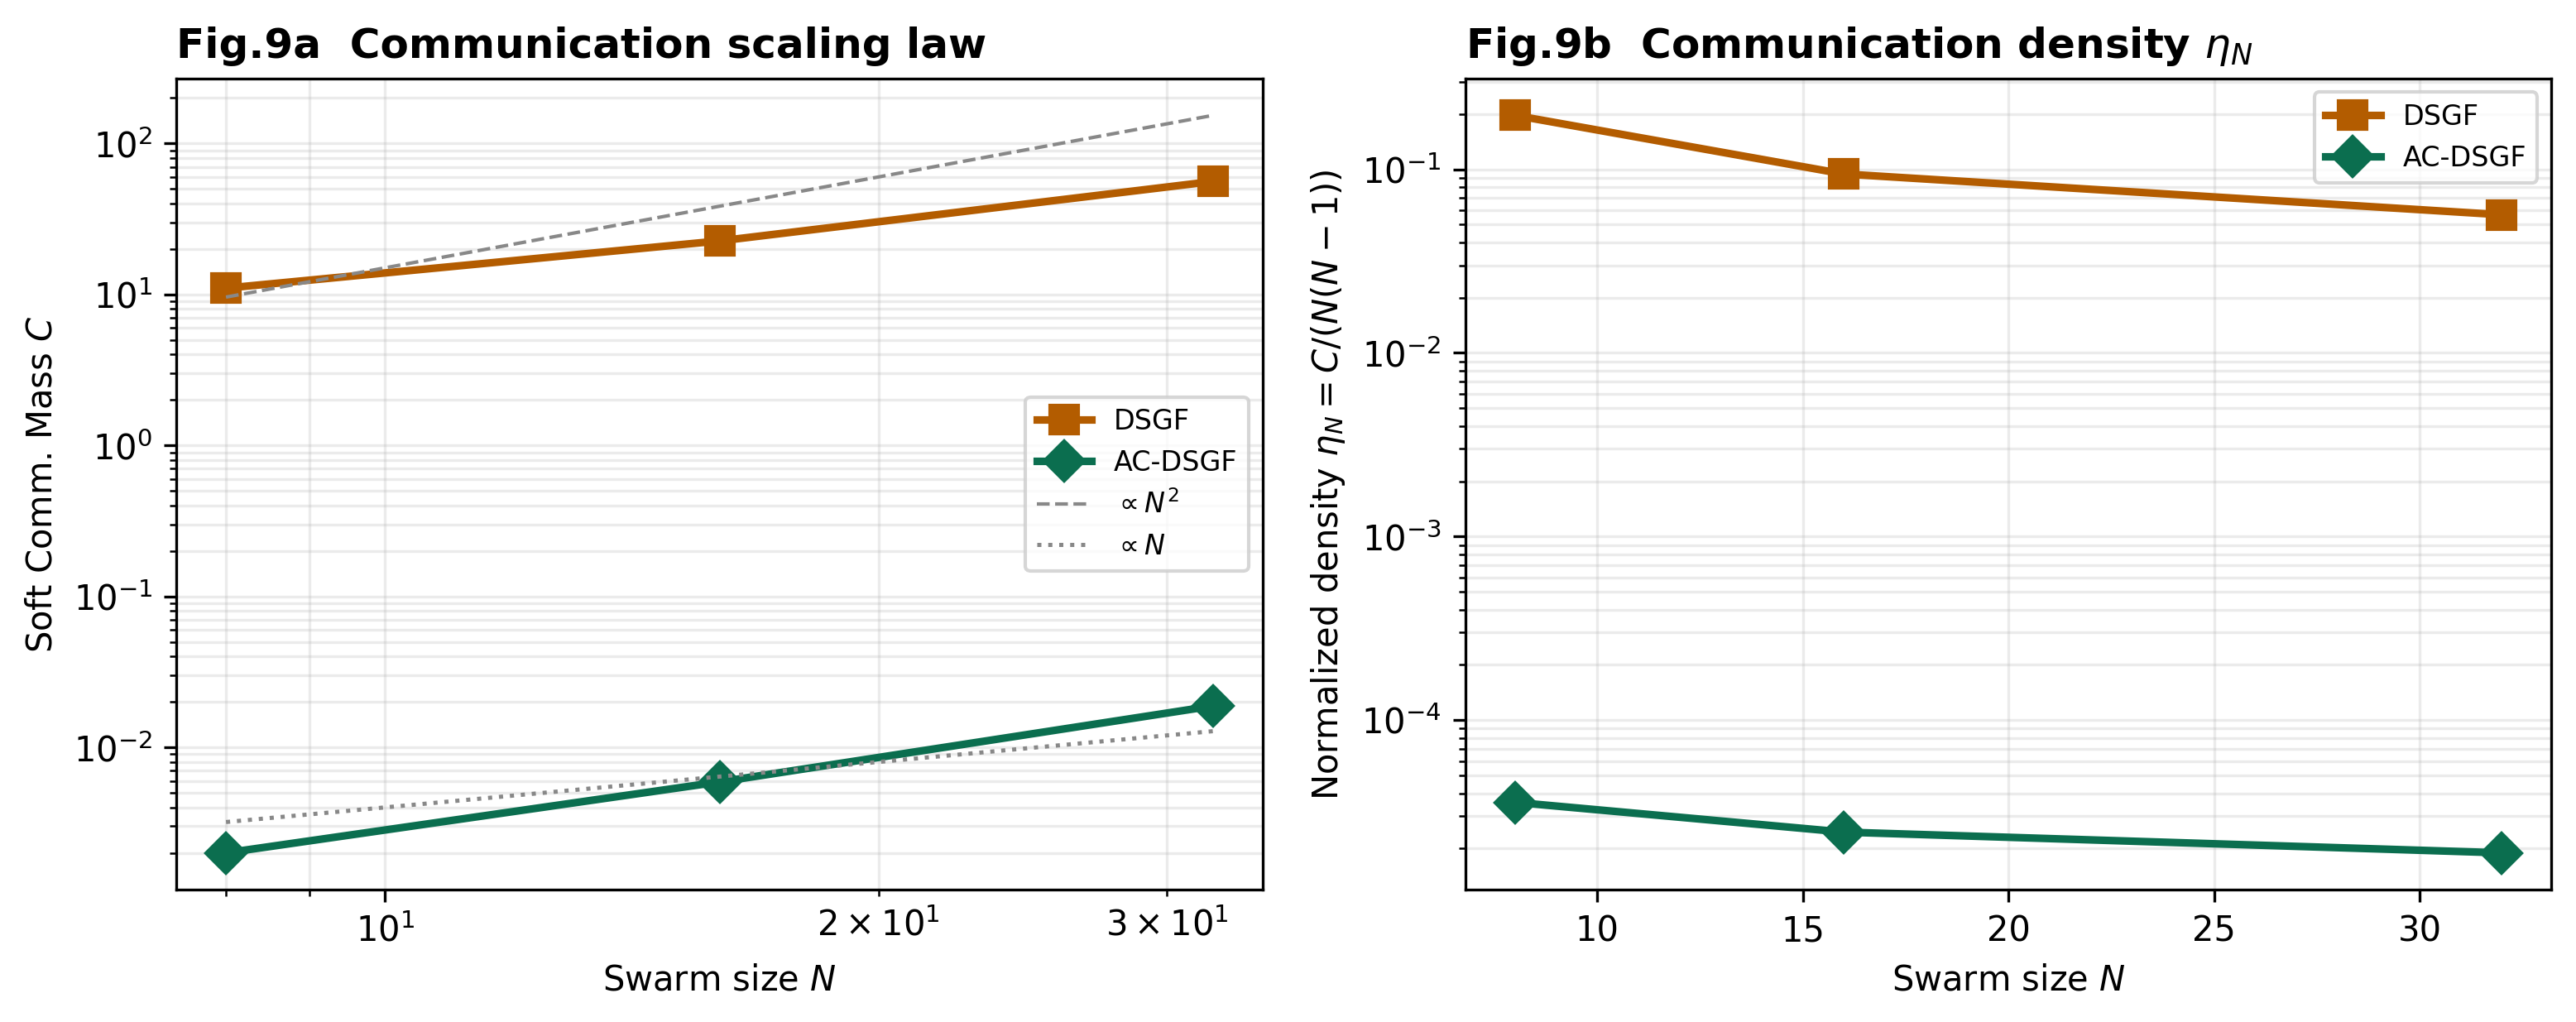
\includegraphics[width=0.98\linewidth]{figures/Fig9_comm_density_scaling.png}
  \caption{Communication density scaling with swarm size.
  AC-DSGF maintains nearly constant sparse activation density as $N$
  increases, while DSGF exhibits much higher interaction density---consistent
  with $\eta_N=\mathcal{O}(K/N)$ (Prop.~2).
  The claim is a different communication growth law, not higher Success at
  $N{=}32$.}
  \label{fig:density-scale}
\end{figure}

\subsubsection{Learned Communication Selectivity}
\label{sec:gate-dist}

\begin{figure}[t]
  \centering
  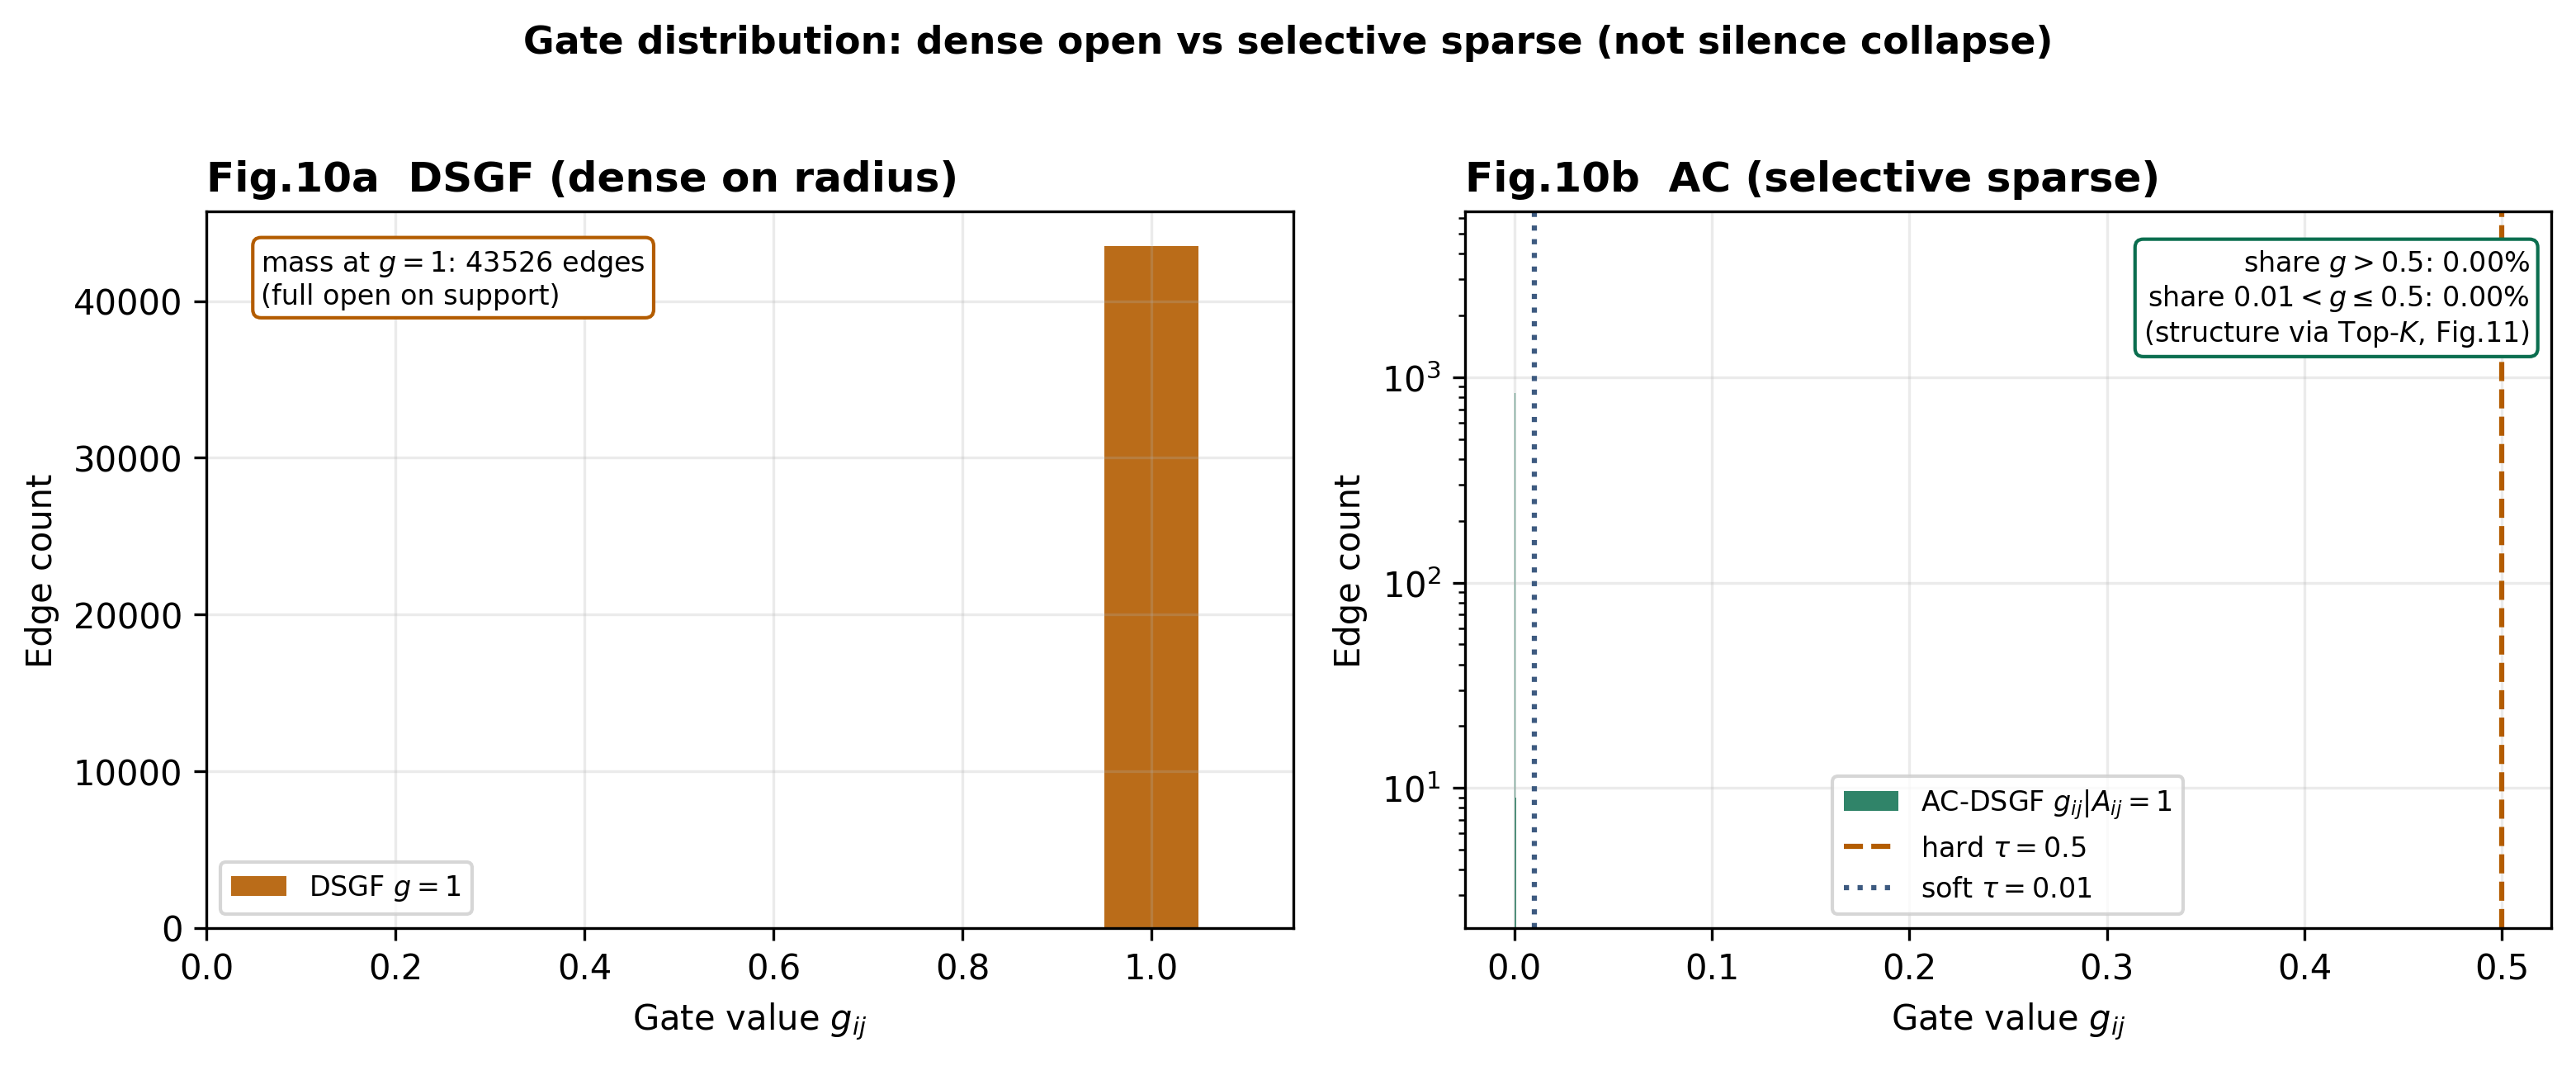
\includegraphics[width=0.98\linewidth]{figures/Fig10_gate_distribution.png}
  \caption{Learned communication selectivity ($N{=}16$).
  (a)~DSGF opens radius edges at $g\equiv1$.
  (b)~AC-DSGF concentrates mass on continuous low-intensity activations rather
  than silencing all edges ($g\equiv0$).
  Structure is evidenced by relative ranking under Top-$K$
  (Fig.~\ref{fig:topk}).}
  \label{fig:gate-dist}
\end{figure}

\subsubsection{Top-$K$ Deployment}
\label{sec:topk-deploy}

\begin{table}[t]
\centering
\caption{Top-$K$ deployment from soft gates ($N{=}16$, eval-only
discretization, no retraining).}
\label{tab:topk}
\begin{tabular}{lc}
\toprule
Deployment rule & Success (\%) \\
\midrule
Soft gate (training-consistent) & $25.8$ \\
Top-1 & $24.5$ \\
Top-2 & $28.1$ \\
Top-3 & $29.4$ \\
\bottomrule
\end{tabular}
\end{table}

\begin{figure}[t]
  \centering
  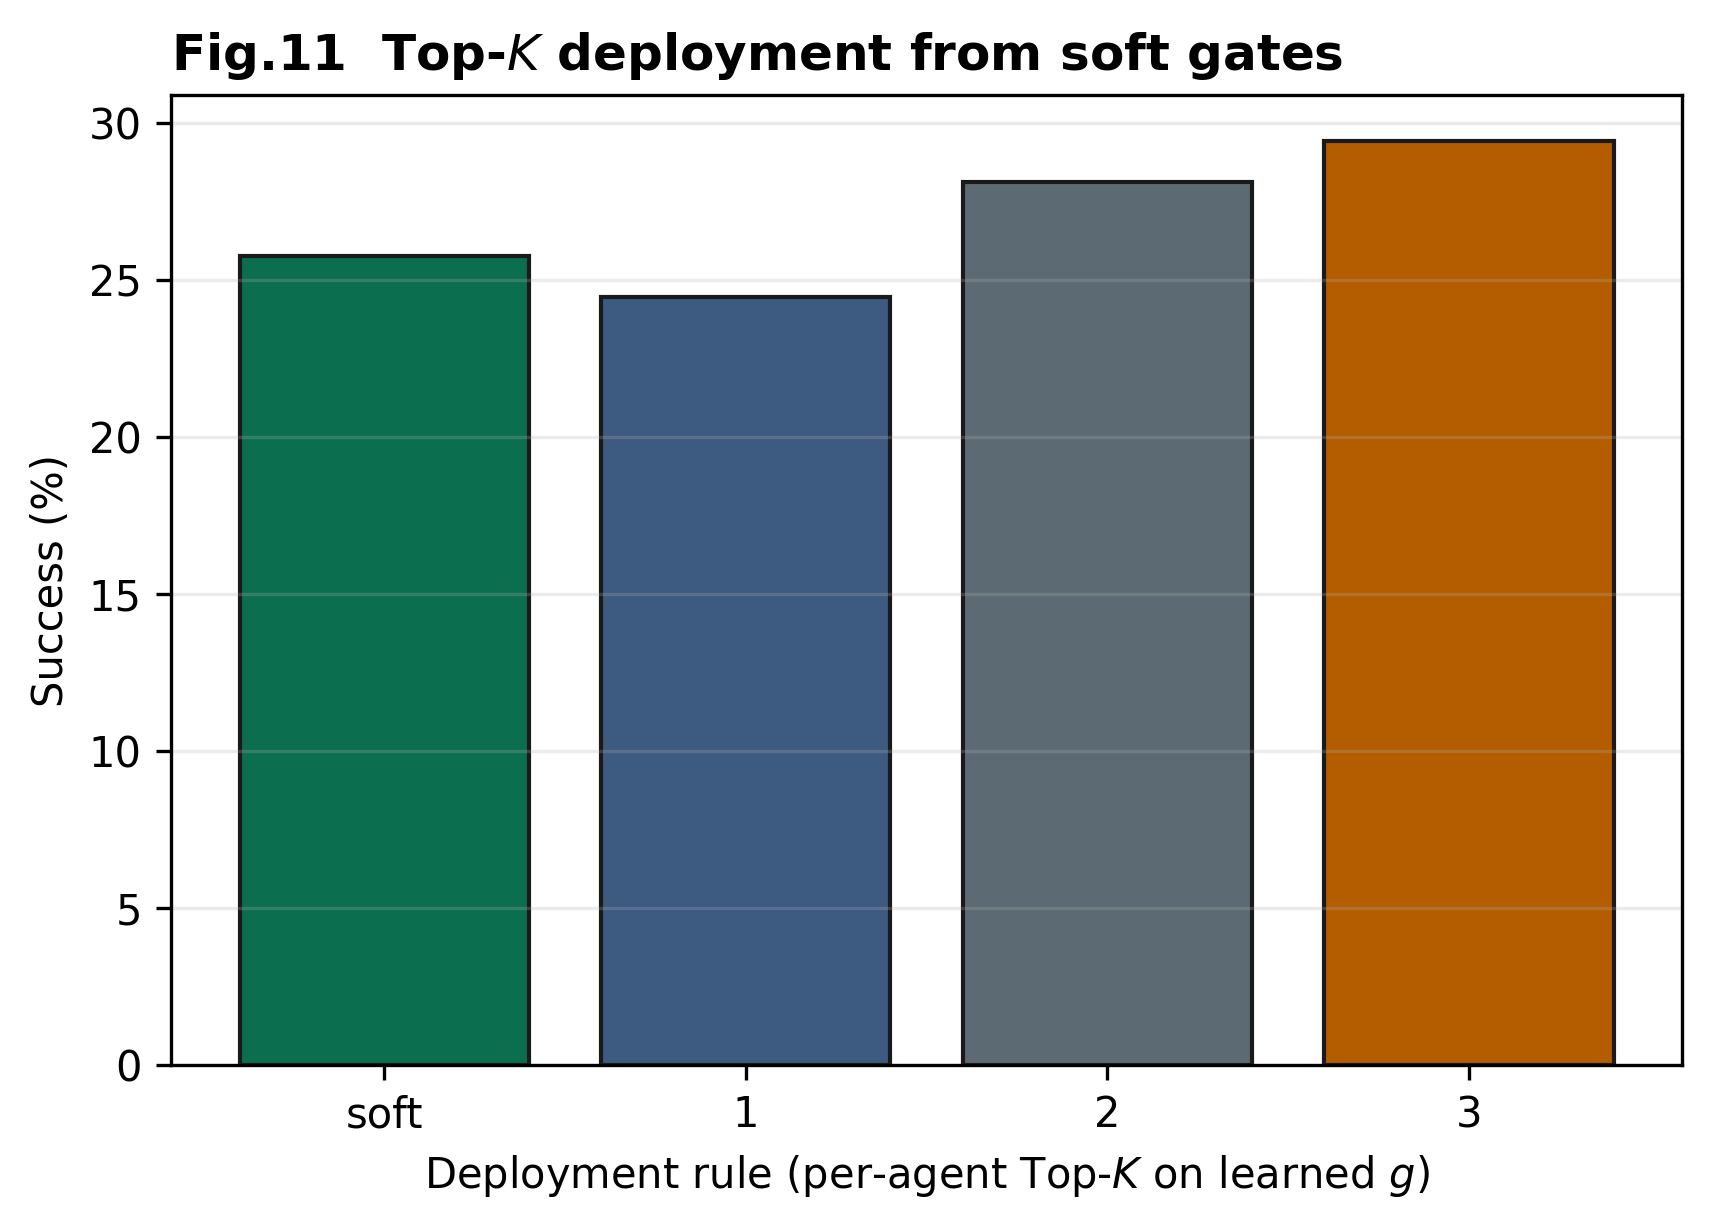
\includegraphics[width=0.72\linewidth]{figures/Fig11_topk_deploy.png}
  \caption{Top-$K$ deployment from soft gates.
  Soft learned topology can be discretized into practical communication links
  at comparable task effectiveness.
  Mild improvements after removing weak soft activations indicate that low-
  confidence edges may inject unnecessary interactions at inference; we do
  \emph{not} claim Top-$K$ should replace soft training.}
  \label{fig:topk}
\end{figure}

\subsection{Robustness under Packet Loss}
\label{sec:packet-loss}

\begin{figure}[t]
  \centering
  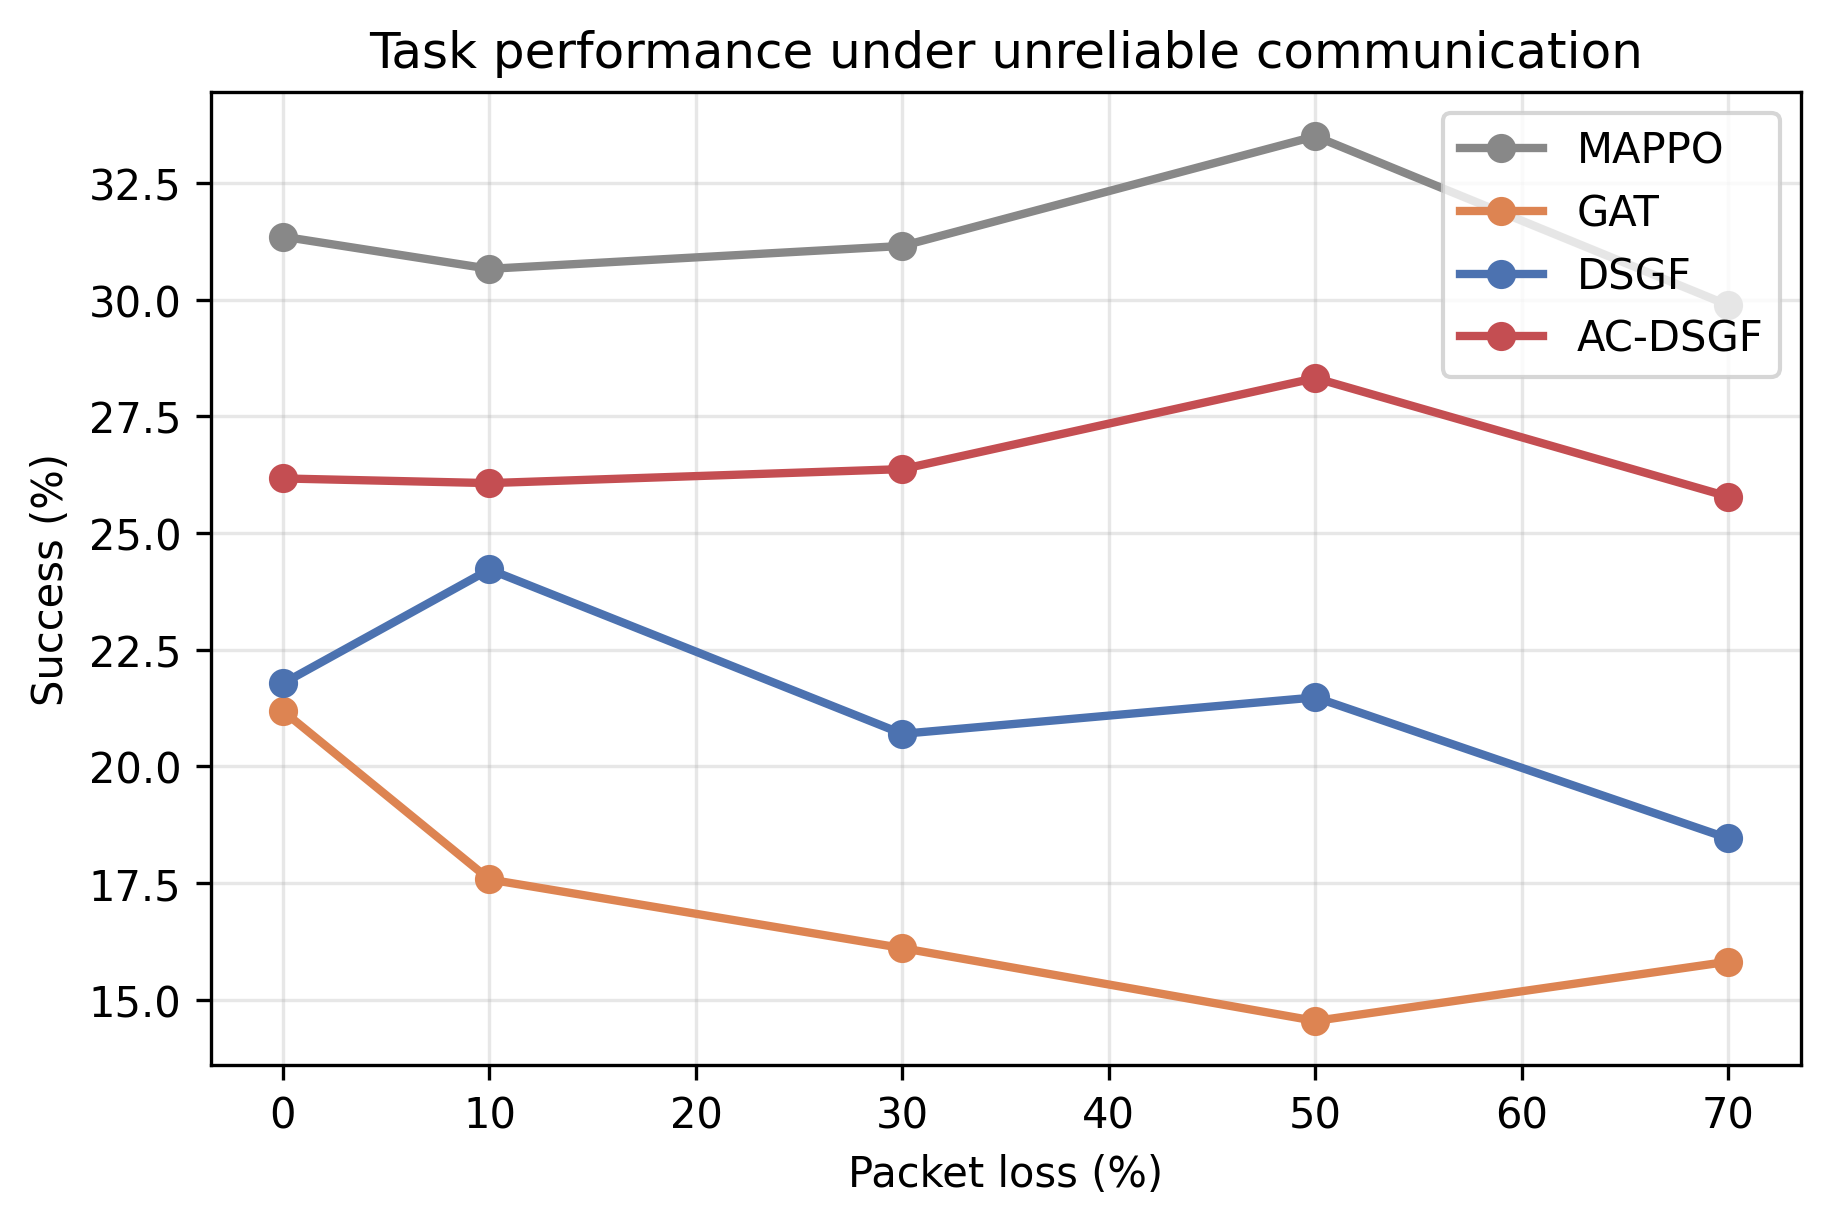
\includegraphics[width=0.85\linewidth]{figures/fig_packet_loss.png}
  \caption{Task success under random edge drops ($N{=}16$).
  AC-DSGF remains nearly flat as loss increases---consistent with
  \emph{graceful degradation} under unreliable links.}
  \label{fig:packet-loss}
\end{figure}

\begin{table}[t]
\centering
\caption{Success (\%) vs.\ packet-loss rate $p$ ($N{=}16$).
Emphasize degradation slope, not absolute comparison to Table~I.}
\label{tab:packet-loss}
\begin{tabular}{lccccc}
\toprule
Method & $0\%$ & $10\%$ & $30\%$ & $50\%$ & $70\%$ \\
\midrule
MAPPO & $31.4$ & $30.7$ & $31.2$ & $33.5$ & $29.9$ \\
GAT & $21.2$ & $17.6$ & $16.1$ & $14.6$ & $15.8$ \\
DSGF & $21.8$ & $24.2$ & $20.7$ & $21.5$ & $18.5$ \\
AC-DSGF & $26.2$ & $26.1$ & $26.4$ & $28.3$ & $25.8$ \\
\bottomrule
\end{tabular}
\end{table}

\subsection{Communication--Performance Pareto}
\label{sec:pareto}

\begin{figure}[t]
  \centering
  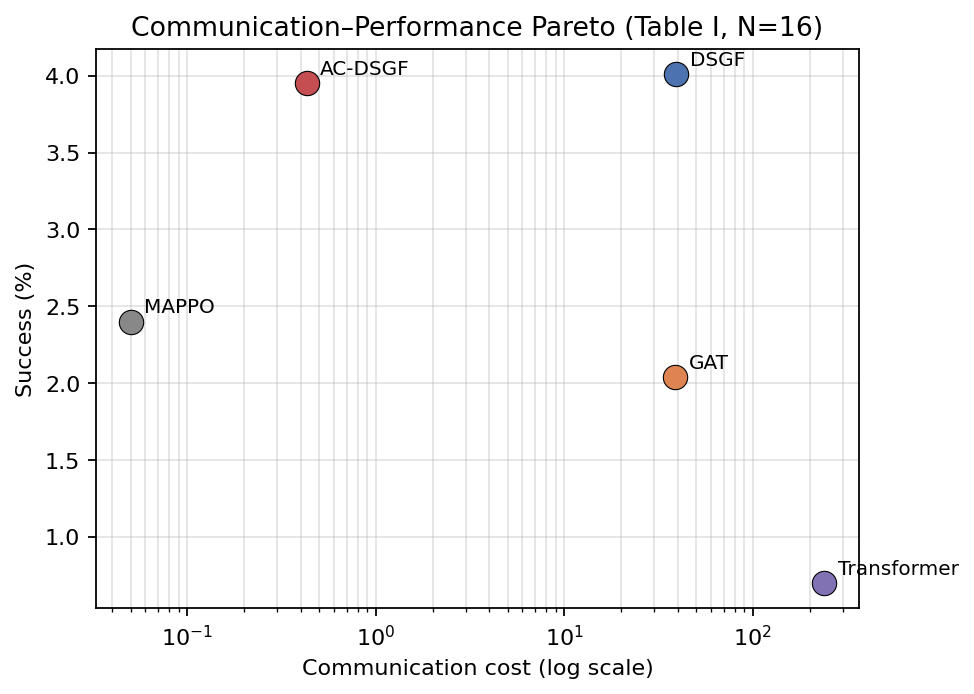
\includegraphics[width=0.70\linewidth]{figures/fig_comm_pareto.png}
\caption{Communication--performance Pareto ($N{=}16$, Table~\ref{tab:main}).
AC-DSGF occupies the high-efficiency region: comparable task effectiveness at
minimal Soft Comm.\ Mass.}
\label{fig:pareto}
\end{figure}


\section*{Discussion and Limitations}
\label{sec:limitations}

AC-DSGF's contribution is \textbf{adaptive topology learning} with a scalable
sparse structure ($\eta_N=\mathcal{O}(K/N)$) and deployable discretization---not
merely reporting a lower Soft Mass number.
Reported $C=\sum g_{ij}$ is a soft intensity proxy, not a physical packet
counter; mapping to radio frames is left to hardware deployment.
Absolute Success remains modest in this navigation benchmark for all methods;
claims are comparative and communication-centric.
Current evaluation focuses on simulation-based multi-agent navigation.
Real-world communication uncertainty, latency, and packet-level constraints
will be investigated in future hardware experiments.
We do not advocate replacing soft gates during training by hard Top-$K$;
discretization is a deployment approximation (Sec.~\ref{sec:theory-deploy}).
